%%%%%%%%%%%%%%%%%%%%%%%%%%%%%%%%%%%%%%%%%%%%%%%%%%%%%%%%%%%%%%%%%%%%%%
% Problem statement
\begin{statement}[
  problempoints=110,
  timelimit=1 sekunda,
  memorylimit=512 MiB,
]{Konstrukcija}

%\setlength\intextsep{-0.1cm}
%\begin{wrapfigure}[7]{r}{0.27\textwidth}
%\centering
%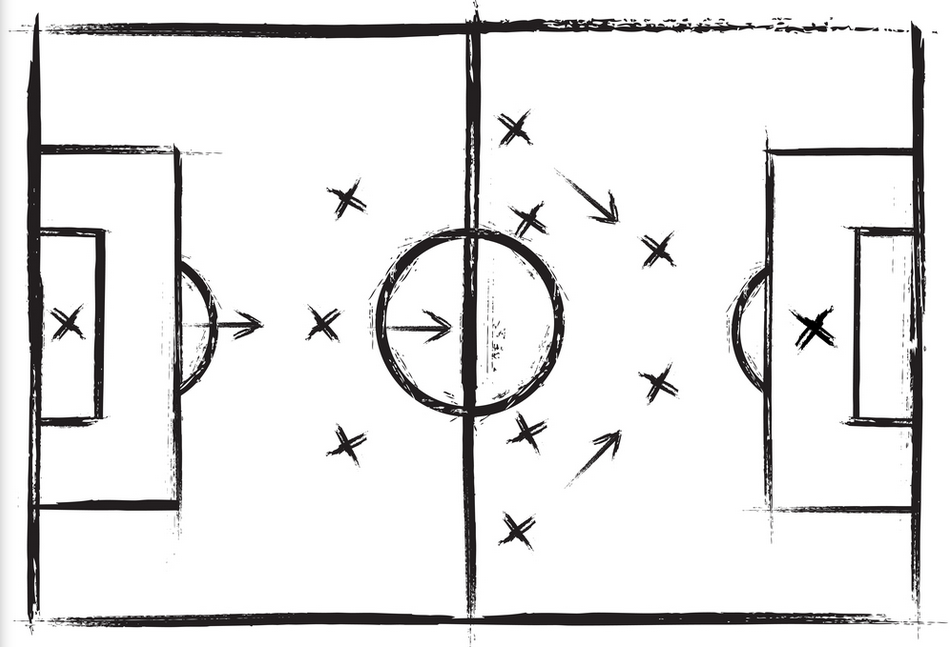
\includegraphics[width=0.27\textwidth]{img/trener.png}
%\end{wrapfigure}

Neka je $G$ usmjereni graf bez ciklusa. Ako su $c_1, c_2, c_3, \dots c_n$
različiti čvorovi grafa $G$ takvi da postoji put od $c_1$ do $c_2$, postoji
put od $c_2$ do $c_3$, \dots i postoji put od $c_{n-1}$ do $c_n$, kažemo da
je niz $C = (c_1, c_2, c_3, \dots c_n)$ uređeni niz koji počinje u čvoru
$c_1$ i završava u čvoru $c_n$. Primijetite da između susjednih elemenata
$c_i$ i $c_{i+1}$ uređenog niza ne moraju postojati direktni bridovi, nego je
dovoljno da postoji put od $c_i$ do $c_{i+1}$.

Za tako definiran uređeni niz $C = (c_1, c_2, c_3, \dots c_n)$, definiramo
njegovu duljinu $len(C) = n$.  Dakle, duljina uređenog niza je jednaka broju
čvorova u uređenom nizu.  Primijetite da uređeni niz može imati duljinu $1$,
tj. da se uređeni niz može sastojati od samo jednog čvora koji je ujedno i
početak i kraj tog uređenog niza.

Također, za uređeni niz $C = (c_1, c_2, c_3, \dots c_n)$ definiramo
njegov predznak kao $sgn(C) = (-1)^{len(C)+1}$.  Za čvorove $x$ i $y$ grafa
$G$, označimo sa $S_{x,y}$ skup svih uređenih nizova koji počinju u $x$ i
završavaju u $y$.

Tada definiramo napetost između čvorova $x$ i $y$ kao $tns(x, y)=\sum_{C \in
S_{x, y}}{sgn(C)}$, tj.\ napetost između čvorova $x$ i $y$ jednaka je zbroju
predznaka svih uređenih nizova koji počinju u $x$ i završavaju u $y$.

Zadan je cijeli broj $K$. Vaš je zadatak konstruirati usmjereni graf bez
ciklusa čiji broj čvorova \textbf{ne prelazi 1000} i čiji broj bridova
također \textbf{ne prelazi 1000} i za koji vrijedi $tns(1, N) = K$, gdje je
$N$ broj čvorova tog konstruiranog grafa i oznake čvorova su prirodni brojevi
$1$, $2$, \dots, $N$.

%%%%%%%%%%%%%%%%%%%%%%%%%%%%%%%%%%%%%%%%%%%%%%%%%%%%%%%%%%%%%%%%%%%%%%
% Input
\subsection*{Ulazni podaci}
U prvom se retku nalazi cijeli broj $K$ $(|K| \le 10^{18})$, iz
teksta zadatka.

%%%%%%%%%%%%%%%%%%%%%%%%%%%%%%%%%%%%%%%%%%%%%%%%%%%%%%%%%%%%%%%%%%%%%%
% Output
\subsection*{Izlazni podaci}
U prvom retku redom treba ispisati broj čvorova i broj bridova konstruiranog
grafa iz teksta zadatka. Označimo broj čvorova tog grafa s $N$ $(1 \le N \le
1000)$, a broj bridova s $M$ $(0 \le M \le 1000)$.

U $i$-tom od sljedećih $M$ redaka redom treba ispisati dva različita prirodna
broja $X_i$ i $Y_i$ $(1 \le X_i, Y_i \le N)$, koji nam predstavljaju $i$-ti
brid koji je usmjeren s čvora $X_i$ u čvor $Y_i$. Svaki brid smije biti
ispisan najviše jednom.

Također, apsolutna vrijednost napetosti između svaka dva čvora u grafu mora
biti manja ili jednaka $2^{80}$.

Ako postoji više mogućih rješenja, ispišite bilo koje.

%%%%%%%%%%%%%%%%%%%%%%%%%%%%%%%%%%%%%%%%%%%%%%%%%%%%%%%%%%%%%%%%%%%%%%
% Scoring
\subsection*{Bodovanje}
{\renewcommand{\arraystretch}{1.4}
  \setlength{\tabcolsep}{6pt}
  \begin{tabular}{ccl}
 Podzadatak & Broj bodova & Ograničenja \\ \midrule
  1 & 15 & $1 \le K < 500$ \\
  2 & 15 & $-300 < N \le 1$ \\
  3 & 20 & $|K| < 10000$\\
  4 & 60 & Nema dodatnih ograničenja. \\
\end{tabular}}

%%%%%%%%%%%%%%%%%%%%%%%%%%%%%%%%%%%%%%%%%%%%%%%%%%%%%%%%%%%%%%%%%%%%%%
% Examples
\subsection*{Probni primjeri}
\begin{tabularx}{\textwidth}{X'X'X}
\sampleinputs{test/konstrukcija.dummy.in.1}{test/konstrukcija.dummy.out.1} &
\sampleinputs{test/konstrukcija.dummy.in.2}{test/konstrukcija.dummy.out.2} &
\sampleinputs{test/konstrukcija.dummy.in.3}{test/konstrukcija.dummy.out.3}
\end{tabularx}

\textbf{Pojašnjenje prvog probnog primjera:}
Konstruirani graf ima $6$ čvorova. Uređeni nizovi koji počinju u $1$ i
završavaju u $6$ su: $(1, 6)$, $(1, 4, 6)$, $(1, 5, 6)$, $(1, 3, 6)$, $(1, 2,
6)$, $(1, 4, 3, 6)$, $(1, 4, 2, 6)$, $(1, 5, 3, 6)$, $(1, 5, 2, 6)$, $(1, 3, 2,
6)$, $(1, 4, 3, 2, 6)$, $(1, 5, 3, 2, 6)$.  Njihove duljine su redom $1, 2, 2,
2, 2, 3, 3, 3, 3, 3, 4, 4$, pa su njihovi predznaci redom $-1, 1, 1, 1, 1, -1,
-1, -1, -1, -1, 1, 1$, pa je napetost između čvorova $1$ i $6$ jednaka $-1 + 1
+ 1 + 1 + 1 - 1 - 1 - 1 - 1 - 1 + 1 + 1 = 0$.

\setlength\intextsep{-0.5cm}
\begin{wrapfigure}{c}{\textwidth}
\centering
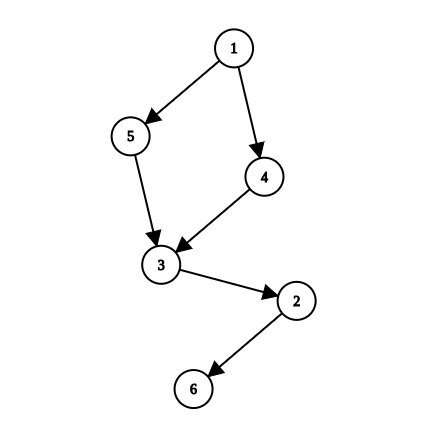
\includegraphics[width=0.6\textwidth]{graph.png}
\end{wrapfigure}

%%%%%%%%%%%%%%%%%%%%%%%%%%%%%%%%%%%%%%%%%%%%%%%%%%%%%%%%%%%%%%%%%%%%%%
% We're done
\end{statement}

%%% Local Variables:
%%% mode: latex
%%% mode: flyspell
%%% ispell-local-dictionary: "croatian"
%%% TeX-master: "../hio.tex"
%%% End:
